\documentclass{extbook}[14pt]
\usepackage{multicol, enumerate, enumitem, hyperref, color, soul, setspace, parskip, fancyhdr, amssymb, amsthm, amsmath, bbm, latexsym, units, mathtools}
\everymath{\displaystyle}
\usepackage[headsep=0.5cm,headheight=0cm, left=1 in,right= 1 in,top= 1 in,bottom= 1 in]{geometry}
\pagestyle{fancy}
\lhead{}
\chead{Answer Key for Module\,6\,-\,Polynomial\,Functions Version B}
\rhead{}
\lfoot{Summer\,C\,2020}
\cfoot{}
\rfoot{}
\begin{document}
\textbf{This key should allow you to understand why you choose the option you did (beyond just getting a question right or wrong). \href{https://xronos.clas.ufl.edu/mac1105spring2020/courseDescriptionAndMisc/Exams/LearningFromResults}{More instructions on how to use this key can be found here}.}

\textbf{If you have a suggestion to make the keys better, \href{https://forms.gle/CZkbZmPbC9XALEE88}{please fill out the short survey here}.}

\textit{Note: This key is auto-generated and may contain issues and/or errors. The keys are reviewed after each exam to ensure grading is done accurately. If there are issues (like duplicate options), they are noted in the offline gradebook. The keys are a work-in-progress to give students as many resources to improve as possible.}

\rule{\textwidth}{0.4pt}

1. Describe the zero behavior of the zero $x = 9$ of the polynomial below.
\[ f(x) = 9(x + 5)^{8}(x - 5)^{4}(x - 9)^{11}(x + 9)^{6} \] 

 
 The solution is  
 \begin{center} 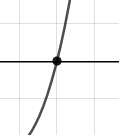
\includegraphics[width=0.3\textwidth]{../Figures/polyZeroBehaviorDB.png} \end{center}\begin{tabular}{|c|c|} 
\hline 
 & \tabularnewline 
 \textbf{A.} 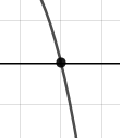
\includegraphics[width=0.3\textwidth]{../Figures/polyZeroBehaviorAB.png} & \textbf{B.} 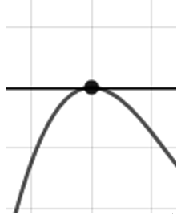
\includegraphics[width=0.3\textwidth]{../Figures/polyZeroBehaviorBB.png} \tabularnewline 
\hline 
 & \tabularnewline 
 \textbf{C.} 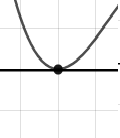
\includegraphics[width=0.3\textwidth]{../Figures/polyZeroBehaviorCB.png} & \textbf{D.} 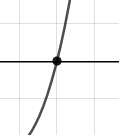
\includegraphics[width=0.3\textwidth]{../Figures/polyZeroBehaviorDB.png} \tabularnewline 
\hline 
 E. None of the figures above. & \tabularnewline 
\hline 
 \end{tabular} 
 
\begin{enumerate}[label=\Alph*.] 
\item   
\item   
\item   
\item   
\end{enumerate} 
 
\textbf{General Comment:} \textbf{General Comments:} You will need to sketch the entire graph, then zoom in on the zero the question asks about. 

-----------------------------------------------

2. Which of the following equations \textit{could} be of the graph presented below?
\begin{center} 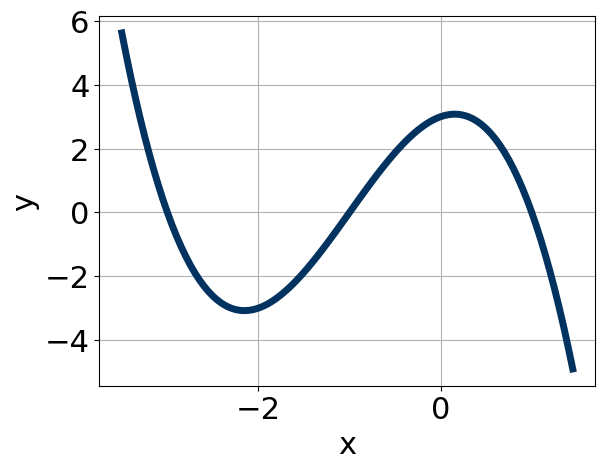
\includegraphics[width=0.3\textwidth]{../Figures/polyGraphToFunctionB.png} \end{center} 

The solution is $ -13(x + 1)^{8} (x + 4)^{5} (x - 2)^{9} $ 

\begin{enumerate}[label=\Alph*.] 
\item $ -2(x + 1)^{9} (x + 4)^{8} (x - 2)^{7} $ 

 The factor $-1$ should have an even power and the factor $-4$ should have an odd power. 
\item $ -10(x + 1)^{8} (x + 4)^{8} (x - 2)^{5} $ 

 The factor $(x + 4)$ should have an odd power. 
\item $ -13(x + 1)^{8} (x + 4)^{5} (x - 2)^{9} $ 

 * This is the correct option. 
\item $ 14(x + 1)^{4} (x + 4)^{9} (x - 2)^{4} $ 

 The factor $(x - 2)$ should have an odd power and the leading coefficient should be the opposite sign. 
\item $ 13(x + 1)^{6} (x + 4)^{9} (x - 2)^{7} $ 

 This corresponds to the leading coefficient being the opposite value than it should be. 
\end{enumerate} 
 
\textbf{General Comment:} General Comments: Draw the x-axis to determine which zeros are touching (and so have even multiplicity) or cross (and have odd multiplicity). 

-----------------------------------------------

3. Describe the end behavior of the polynomial below.
\[ f(x) = -4(x + 3)^{4}(x - 3)^{5}(x + 8)^{4}(x - 8)^{5} \] 

 
 The solution is  
 \begin{center} 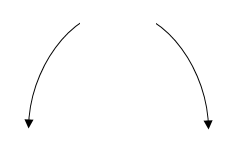
\includegraphics[width=0.3\textwidth]{../Figures/polyEndBehaviorBB.png} \end{center}\begin{tabular}{|c|c|} 
\hline 
 & \tabularnewline 
 \textbf{A.} 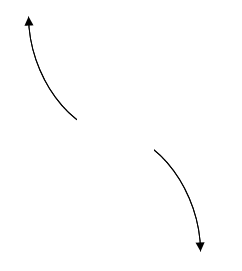
\includegraphics[width=0.3\textwidth]{../Figures/polyEndBehaviorAB.png} & \textbf{B.} 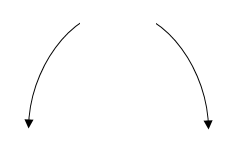
\includegraphics[width=0.3\textwidth]{../Figures/polyEndBehaviorBB.png} \tabularnewline 
\hline 
 & \tabularnewline 
 \textbf{C.} 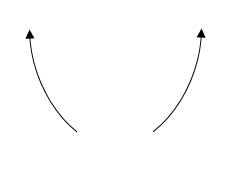
\includegraphics[width=0.3\textwidth]{../Figures/polyEndBehaviorCB.png} & \textbf{D.} 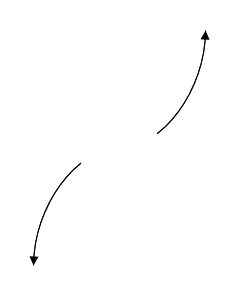
\includegraphics[width=0.3\textwidth]{../Figures/polyEndBehaviorDB.png} \tabularnewline 
\hline 
 E. None of the figures above. & \tabularnewline 
\hline 
 \end{tabular} 
 
\begin{enumerate}[label=\Alph*.] 
\item The function is above the $x$-axis, then passes through.  
\item The function is below the $x$-axis, then touches.  
\item The function is above the $x$-axis, then touches.  
\item The function is below the $x$-axis, then passes through.  
\end{enumerate} 
 
\textbf{General Comment:} \textbf{General Comments:} Remember that end behavior is determined by the leading coefficient AND whether the \textbf{sum} of the multiplicities is positive or negative. 

-----------------------------------------------

4. Construct the lowest-degree polynomial given the zeros below. Then, choose the intervals that contain the coefficients of the polynomial in the form $ax^3+bx^2+cx+d$.
\[ \frac{-7}{5}, \frac{7}{3}, \text{ and } \frac{-2}{3} \] 
The solution is $ 45x^{3} -12 x^{2} -175 x -98 $ 

\begin{enumerate}[label=\Alph*.] 
\item $ a \in [35, 48], b \in [6, 14], c \in [-180, -167], \text{ and } d \in [93, 104] $ 

 $45x^{3} +12 x^{2} -175 x + 98$, which corresponds to multiplying out $(5x -7)(3x + 7)(3x -2)$. 
\item $ a \in [35, 48], b \in [-14, -6], c \in [-180, -167], \text{ and } d \in [-100, -90] $ 

 * $45x^{3} -12 x^{2} -175 x -98$, which is the correct option. 
\item $ a \in [35, 48], b \in [-141, -136], c \in [30, 43], \text{ and } d \in [93, 104] $ 

 $45x^{3} -138 x^{2} +35 x + 98$, which corresponds to multiplying out $(5x + 5)(3x -3)(3x -3)$. 
\item $ a \in [35, 48], b \in [71, 76], c \in [-126, -112], \text{ and } d \in [-100, -90] $ 

 $45x^{3} +72 x^{2} -119 x -98$, which corresponds to multiplying out $(5x + 5)(3x + 3)(3x -3)$. 
\item $ a \in [35, 48], b \in [-14, -6], c \in [-180, -167], \text{ and } d \in [93, 104] $ 

 $45x^{3} -12 x^{2} -175 x + 98$, which corresponds to multiplying everything correctly except the constant term. 
\end{enumerate} 
 
\textbf{General Comment:} General Comments: To construct the lowest-degree polynomial, you want to multiply out $(5x + 7)(3x -7)(3x + 2)$ 

-----------------------------------------------

0. Construct the lowest-degree polynomial given the zeros below. Then, choose the intervals that contain the coefficients of the polynomial in the form $x^3+bx^2+cx+d$.
\[ 4 + 2 i \text{ and } x -3 \] 
The solution is $ x^{3} -5 x^{2} -4 x + 60 $ 

\begin{enumerate}[label=\Alph*.] 
\item $ b \in [-6.9, -3.4], c \in [-9.6, -2.8], \text{ and } d \in [57, 63] $ 

 * $x^{3} -5 x^{2} -4 x + 60$, which is the correct option. 
\item $ b \in [0.7, 1.6], c \in [-2.7, -0.1], \text{ and } d \in [-17, -7] $ 

 $x^{3} + x^{2} -x -12$, which corresponds to multiplying out $(x -4)(x + 3)$. 
\item $ b \in [0.7, 1.6], c \in [0.2, 2.5], \text{ and } d \in [-7, -2] $ 

 $x^{3} + x^{2} +x -6$, which corresponds to multiplying out $(x -2)(x + 3)$. 
\item $ b \in [3.6, 7.9], c \in [-9.6, -2.8], \text{ and } d \in [-67, -52] $ 

 $x^{3} +5 x^{2} -4 x -60$, which corresponds to multiplying out $(x-(4 + 2 i))(x-(4 - 2 i))(x -3)$. 
\item $ \text{None of the above.} $ 

 This corresponds to making an unanticipated error or not understanding how to use nonreal complex numbers to create the lowest-degree polynomial. If you chose this and are not sure what you did wrong, please contact the coordinator for help. 
\end{enumerate} 
 
\textbf{General Comment:} Remember that the conjugate of $a+bi$ is $a-bi$. Since these zeros always come in pairs, we need to multiply out $(x-(4 + 2 i))(x-(4 - 2 i))(x-(x -3))$. 

-----------------------------------------------


\end{document}

